% Created by tikzDevice version 0.7.0 on 2015-05-24 13:23:23
% !TEX encoding = UTF-8 Unicode
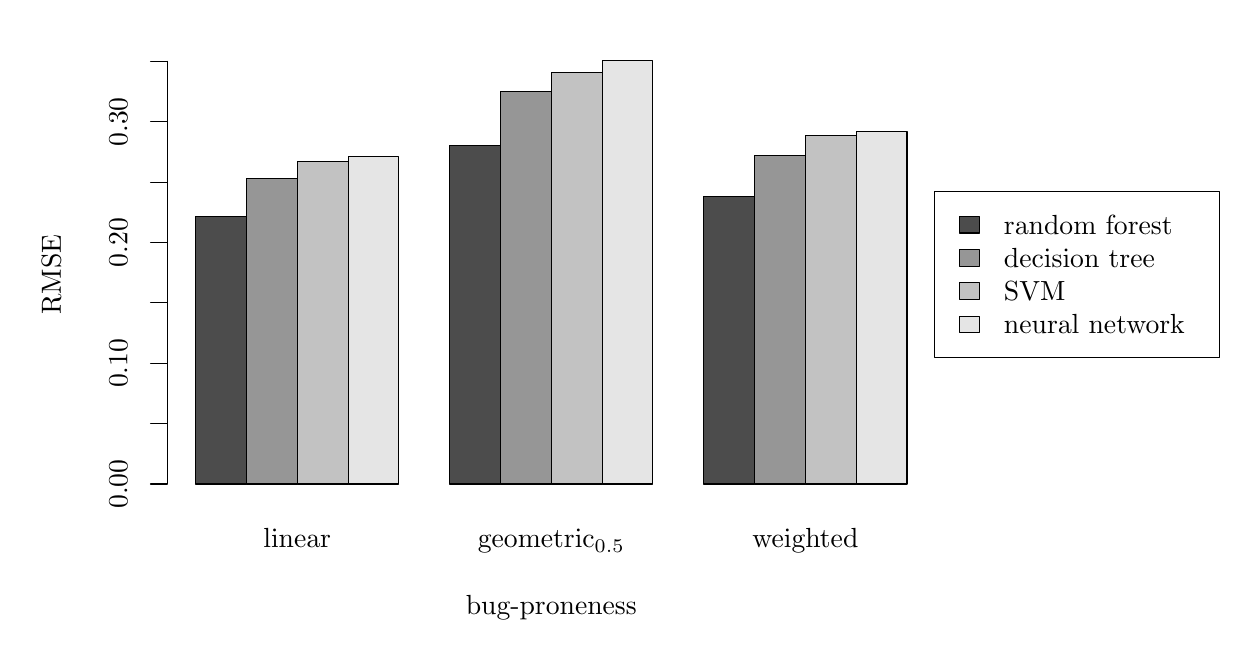
\begin{tikzpicture}[x=1pt,y=1pt]
\definecolor[named]{fillColor}{rgb}{1.00,1.00,1.00}
\path[use as bounding box,fill=fillColor,fill opacity=0.00] (0,0) rectangle (433.62,216.81);
\begin{scope}
\path[clip] (  0.00,  0.00) rectangle (433.62,216.81);
\definecolor[named]{drawColor}{rgb}{0.00,0.00,0.00}
\definecolor[named]{fillColor}{rgb}{0.30,0.30,0.30}

\path[draw=drawColor,line width= 0.4pt,line join=round,line cap=round,fill=fillColor] ( 60.68, 51.93) rectangle ( 79.04,148.63);
\definecolor[named]{fillColor}{rgb}{0.59,0.59,0.59}

\path[draw=drawColor,line width= 0.4pt,line join=round,line cap=round,fill=fillColor] ( 79.04, 51.93) rectangle ( 97.40,162.44);
\definecolor[named]{fillColor}{rgb}{0.76,0.76,0.76}

\path[draw=drawColor,line width= 0.4pt,line join=round,line cap=round,fill=fillColor] ( 97.40, 51.93) rectangle (115.77,168.44);
\definecolor[named]{fillColor}{rgb}{0.90,0.90,0.90}

\path[draw=drawColor,line width= 0.4pt,line join=round,line cap=round,fill=fillColor] (115.77, 51.93) rectangle (134.13,170.23);
\definecolor[named]{fillColor}{rgb}{0.30,0.30,0.30}

\path[draw=drawColor,line width= 0.4pt,line join=round,line cap=round,fill=fillColor] (152.49, 51.93) rectangle (170.85,174.38);
\definecolor[named]{fillColor}{rgb}{0.59,0.59,0.59}

\path[draw=drawColor,line width= 0.4pt,line join=round,line cap=round,fill=fillColor] (170.85, 51.93) rectangle (189.21,193.71);
\definecolor[named]{fillColor}{rgb}{0.76,0.76,0.76}

\path[draw=drawColor,line width= 0.4pt,line join=round,line cap=round,fill=fillColor] (189.21, 51.93) rectangle (207.57,200.55);
\definecolor[named]{fillColor}{rgb}{0.90,0.90,0.90}

\path[draw=drawColor,line width= 0.4pt,line join=round,line cap=round,fill=fillColor] (207.57, 51.93) rectangle (225.93,204.81);
\definecolor[named]{fillColor}{rgb}{0.30,0.30,0.30}

\path[draw=drawColor,line width= 0.4pt,line join=round,line cap=round,fill=fillColor] (244.29, 51.93) rectangle (262.65,155.88);
\definecolor[named]{fillColor}{rgb}{0.59,0.59,0.59}

\path[draw=drawColor,line width= 0.4pt,line join=round,line cap=round,fill=fillColor] (262.65, 51.93) rectangle (281.02,170.62);
\definecolor[named]{fillColor}{rgb}{0.76,0.76,0.76}

\path[draw=drawColor,line width= 0.4pt,line join=round,line cap=round,fill=fillColor] (281.02, 51.93) rectangle (299.38,177.70);
\definecolor[named]{fillColor}{rgb}{0.90,0.90,0.90}

\path[draw=drawColor,line width= 0.4pt,line join=round,line cap=round,fill=fillColor] (299.38, 51.93) rectangle (317.74,179.34);
\end{scope}
\begin{scope}
\path[clip] (  0.00,  0.00) rectangle (433.62,216.81);
\definecolor[named]{drawColor}{rgb}{0.00,0.00,0.00}

\node[text=drawColor,anchor=base,inner sep=0pt, outer sep=0pt, scale=  1.00] at ( 97.40, 28.80) {linear};

\node[text=drawColor,anchor=base,inner sep=0pt, outer sep=0pt, scale=  1.00] at (189.21, 28.80) {geometric$_{0.5}$};

\node[text=drawColor,anchor=base,inner sep=0pt, outer sep=0pt, scale=  1.00] at (281.02, 28.80) {weighted};
\end{scope}
\begin{scope}
\path[clip] (  0.00,  0.00) rectangle (433.62,216.81);
\definecolor[named]{drawColor}{rgb}{0.00,0.00,0.00}

\path[draw=drawColor,line width= 0.4pt,line join=round,line cap=round] (327.59,157.60) rectangle (430.74, 97.61);
\definecolor[named]{fillColor}{rgb}{0.30,0.30,0.30}

\path[draw=drawColor,line width= 0.4pt,line join=round,line cap=round,fill=fillColor] (336.59,148.61) rectangle (343.79,142.60);
\definecolor[named]{fillColor}{rgb}{0.59,0.59,0.59}

\path[draw=drawColor,line width= 0.4pt,line join=round,line cap=round,fill=fillColor] (336.59,136.61) rectangle (343.79,130.61);
\definecolor[named]{fillColor}{rgb}{0.76,0.76,0.76}

\path[draw=drawColor,line width= 0.4pt,line join=round,line cap=round,fill=fillColor] (336.59,124.61) rectangle (343.79,118.61);
\definecolor[named]{fillColor}{rgb}{0.90,0.90,0.90}

\path[draw=drawColor,line width= 0.4pt,line join=round,line cap=round,fill=fillColor] (336.59,112.60) rectangle (343.79,106.61);

\node[text=drawColor,anchor=base west,inner sep=0pt, outer sep=0pt, scale=  1.00] at (352.79,142.16) {random forest};

\node[text=drawColor,anchor=base west,inner sep=0pt, outer sep=0pt, scale=  1.00] at (352.79,130.16) {decision tree};

\node[text=drawColor,anchor=base west,inner sep=0pt, outer sep=0pt, scale=  1.00] at (352.79,118.16) {SVM};

\node[text=drawColor,anchor=base west,inner sep=0pt, outer sep=0pt, scale=  1.00] at (352.79,106.16) {neural network};

\node[text=drawColor,anchor=base,inner sep=0pt, outer sep=0pt, scale=  1.00] at (189.21,  4.80) {bug-proneness};

\node[text=drawColor,rotate= 90.00,anchor=base,inner sep=0pt, outer sep=0pt, scale=  1.00] at ( 12.00,127.61) {RMSE};
\end{scope}
\begin{scope}
\path[clip] (  0.00,  0.00) rectangle (433.62,216.81);
\definecolor[named]{drawColor}{rgb}{0.00,0.00,0.00}

\path[draw=drawColor,line width= 0.4pt,line join=round,line cap=round] ( 50.40, 51.93) -- ( 50.40,204.58);

\path[draw=drawColor,line width= 0.4pt,line join=round,line cap=round] ( 50.40, 51.93) -- ( 44.40, 51.93);

\path[draw=drawColor,line width= 0.4pt,line join=round,line cap=round] ( 50.40, 73.74) -- ( 44.40, 73.74);

\path[draw=drawColor,line width= 0.4pt,line join=round,line cap=round] ( 50.40, 95.54) -- ( 44.40, 95.54);

\path[draw=drawColor,line width= 0.4pt,line join=round,line cap=round] ( 50.40,117.35) -- ( 44.40,117.35);

\path[draw=drawColor,line width= 0.4pt,line join=round,line cap=round] ( 50.40,139.16) -- ( 44.40,139.16);

\path[draw=drawColor,line width= 0.4pt,line join=round,line cap=round] ( 50.40,160.97) -- ( 44.40,160.97);

\path[draw=drawColor,line width= 0.4pt,line join=round,line cap=round] ( 50.40,182.77) -- ( 44.40,182.77);

\path[draw=drawColor,line width= 0.4pt,line join=round,line cap=round] ( 50.40,204.58) -- ( 44.40,204.58);

\node[text=drawColor,rotate= 90.00,anchor=base,inner sep=0pt, outer sep=0pt, scale=  1.00] at ( 36.00, 51.93) {0.00};

\node[text=drawColor,rotate= 90.00,anchor=base,inner sep=0pt, outer sep=0pt, scale=  1.00] at ( 36.00, 95.54) {0.10};

\node[text=drawColor,rotate= 90.00,anchor=base,inner sep=0pt, outer sep=0pt, scale=  1.00] at ( 36.00,139.16) {0.20};

\node[text=drawColor,rotate= 90.00,anchor=base,inner sep=0pt, outer sep=0pt, scale=  1.00] at ( 36.00,182.77) {0.30};
\end{scope}
\end{tikzpicture}
